\section{A Clustering-Based Method for Automatic Educational Video Recommendation Using Deep Face-Features of Lecturers}

Following the approach described in Section \ref{webmedia}, in \cite{mendes2020ISM}, we used actors face clustering for recommending videos that share the presence of the same actors. 
%%
This work aimed at recommending educational video content based on lecturers' presence.
To do that, we take advantage of face detection methods.
More precisely, we detect lecturers in a video taken as a reference and perform a clustering based on the face of these lecturers in different videos.
Given these clusters, we extract their \textit{centroids} (explained in Section~\ref{sec:ism_method}), and perform another clustering step for creating a relationship between videos that share the presence of the same lecturers.
Finally, we rank the recommended videos based on the amount of time the referenced lecturers were present.
A particular feature of this approach is that it can be done without supervision, allowing for new videos to be automatically analyzed.

%As we obtained the best results with the combination SeNet-50 with Agglomerative Clustering in \cite{mendes2020cluster}, we used this same combination in \cite{mendes2020ISM}. 

\begin{figure}[!ht]
    \centering
    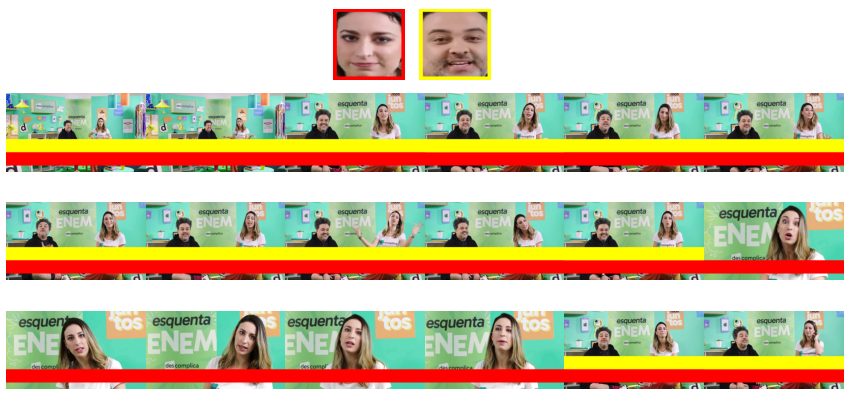
\includegraphics[width=0.75\textwidth]{img/ism/educational_timeline2.png}
    \caption{Timeline with tagged frames by their clusters~(actors) present.}
    \label{fig:timeline2}
\end{figure}



%In that work, we used actors face clustering in 98 videos and around 72\% of the faces went to the correct clusters. Figure \ref{fig:timeline2} shows part of the timeline of one of the videos tagged with colors representing the color of each actor present.


\subsection{Method}
\label{sec:ism_method}

Our method intends to recommend educational videos based on the lecturers that appear in each video, so that, when a person watches a video, other videos containing the same lecturers are recommended.
For didactic purposes we decided to divide our exposition in two phases: (i)~\emph{video representation} and (ii)~\emph{video recommendation}, which are described in Sections~\ref{subsec:video_representation} and \ref{subsec:video_recommendation} respectively.

\subsubsection{Video Representation}
\label{subsec:video_representation}

\begin{figure*}[!ht]
  \centering
  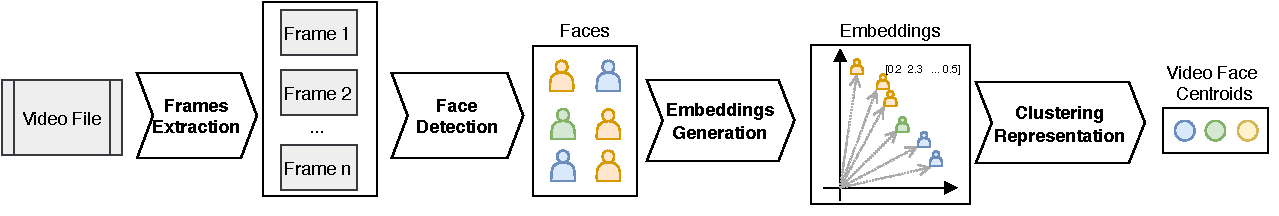
\includegraphics[width=\linewidth]{img/ism/video_clustering_line.pdf}
  \caption{Video representation process with lecturers face centroids. }
  \label{fig:video_clustering}
\end{figure*}

The objective of this phase is to represent each video with vectors~(centroids) of the lecturers that appear on it. 
Fig. \ref{fig:video_clustering} shows the pipeline we propose for this phase, described in the remainder of this subsection.
It is divided into four steps: \emph{Frames Extraction}, \emph{Face Detection}, \emph{Embeddings Generation} and \emph{Clustering Representation}.

The steps of this process are the same used in Figure \ref{fig:cluster_matching} up to the \emph{Face Clustering} step, obtaining the video face clusters.
%%
The difference here is that the \emph{Clustering Representation} returns the centroids of the clusters found.
%%
By the end of this phase, we have each video in the dataset represented by its centroids where, ideally, each centroid represents a lecturer present in the video.


\subsubsection{Video Recommendation}
\label{subsec:video_recommendation}

This phase aims at recommending videos by the lecturers present in it and in the other videos.
It is divided in two steps: \emph{Centroids Clustering} and \emph{Ranking}, as depicted in Fig. \ref{fig:video_recommendation}.

\begin{figure*}[!ht]
  \centering
  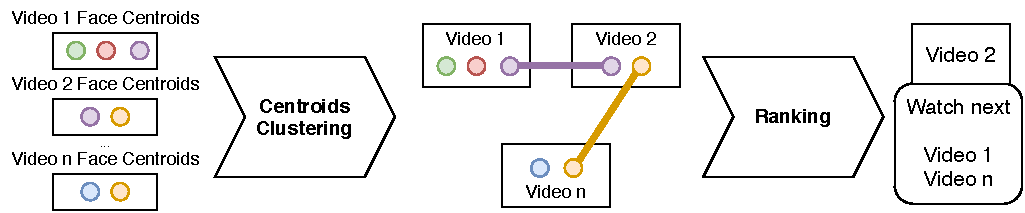
\includegraphics[width=0.8\linewidth]{img/ism/video_recommendation.pdf}
  \caption{Video Recommendation process.}
  \label{fig:video_recommendation}
\end{figure*}

First, we gather the centroids from the videos of the dataset as one single set and perform the \textit{Centroids Clustering}.
%%
By doing that, we group centroids from the same lecturer that are in different videos. For instance, in Fig. \ref{fig:video_recommendation}, one can see that the \emph{purple lecturer} is present in both Videos 1 and 2, while the \emph{orange lecturer} is present in both Videos 2 and n. By the end of this step, we have the group $L$ of lecturers present in the dataset of videos $V$, and we can also denote $L_v$ as the group of lecturers present in video $v$.

Next, based on these relationships among different videos, we perform \textit{Ranking}, by recommending videos in which lecturers of the current video are present. 
%%
For doing that, we compute a similarity score using the presence of the lecturers in the current video and the presence of these same lecturers in the other video.
%%
Let $p_{l,v}$ denote the percentage of frames in which the lecturer $l \in L_v$ is present in video $v \in V$. For each video $v \in V$ and $u \in V-v$ we compute a score of similarity $S_{v,u}$.

\vspace{-1em}
\begin{equation}
  S_{v,u} = \sum_{l~\in~L_v}{p_{l,v}\cdot{p_{l,u}}}
\end{equation}

Finally, using this score, for each video $v$ we compute a ranking $R_{v}$ where $R_{v,i}$ denotes the \emph{i-greatest} $S_v$ and $R_{v,i}\ge~R_{v,i+1}$ for all $i~\in~1...n_v$, where $n_v$ is the number of videos $u$ in which $S_{v,u}>~0$. 
%%
In this way, the more lecturers a video have in common with the reference video, and the more time these lecturers are present in both videos, the higher the video is positioned in the ranking of the reference video.  

By the end of this phase, we have a ranking of recommended videos for each video in the dataset.
%%
It is important to notice that our method is unsupervised and does not require the information of the lecturers in advance.
%%
Consequently, we do not store any information regarding the identity of the lecturers, respecting their privacy.

\subsection{Evaluation}

For representing the video files in the dataset, we start by performing \emph{Frames Extraction} for each video file using a frame rate of 1 frame per second~(fps). 
%%
Next, in the \emph{Face Detection} step, we use MTCNN \cite{mtcnn} (Multitask
Cascaded Convolutional Networks). 
%%
Once we have detected the faces of lecturers in the video frames, we perform \emph{Embeddings Generation} using SeNet-50 \cite{senet}.
%%
Finally, in the \emph{Clustering Representation} step, we used the Ward Agglomerative Clustering~\cite{ward1963hierarchical}.
%%
The choice for the combination SeNet-50 with the Agglomerative Clustering algorithm comes from the fact that this combination returned the best results in the evaluation described in Section \ref{faces_clustering_evaluation}.

For performing the video recommendation task, we gather the centroids~(that represent each lecturer in the video) from all videos in the dataset. Next, we perform the process described in Section \ref{subsec:video_recommendation}.

We evaluate our approach based on the relevance of the videos recommended. A video is considered relevant to another if they have at least one lecturer in common.
%%
To verify that, we use the information of the lecturers' presence available on our dataset.
%%
%%
To evaluate our ranking, for each video we compute the Average Precision~(AP), that evaluates how well a ranking of recommendations is based on each element's relevancy. 
%%
This metric penalizes more a ranking if a non-relevant element is recommended in the first positions than if it was in the last ones.

In order to prevent outliers from having much influence in the recommendation (e.g. a person that is not a lecturer -- and not relevant to the video -- and appears for a short amount of time), we evaluated different thresholds of presence intervals in a video for a person to be considered as ``present'' when computing the score for the ranking. 
%%
In this way, a $p_{l,v}$ lesser than the threshold is considered as $0$.
%%
Besides the Average Precision, we also compute the mean value of the recall~(MeanR), precision~(MeanP), and F1-Score~(MeanF1) for the recommendation generated for each of the videos, without considering the positioning of these videos in the rankings.

One can observe from Table \ref{tab:results} that the precision clearly increased with the use of the threshold.
%%
Different from the precision, the recall decreased with the increase of the threshold. It means that with a greater threshold more videos that should be recommended were not chosen by our method.
%%
It is important to notice that these two metrics~(precision and recall) do not consider the ordering of the recommendations.
%%
Different from them, the Mean Average Precision~(mAP) has high values for all thresholds, especially because the score for computing the ranking takes into consideration the percentage of time that a person appears in the reference and recommended videos.
%%
Then, we can conclude that our proposed approach for ordering the recommended videos tends to recommend more suitable videos first with a high mAP$\approx0.99$.

\begin{table}[!ht]
\small
\centering
\caption{Results with different thresholds of presence.}
\label{tab:results}
\begin{tabular}{ccccccccc}
\hline
\textbf{Thershold} & \textbf{MeanR} & \textbf{MeanP} & \textbf{MeanF1}  & \textbf{mAP} \\ \hline
0\%                & 0,88851        & 0,64681        & 0,70971          & 0,98641      \\
5\%                & 0,88851        & 0,69923        & 0,74930          & 0,98642      \\
10\%               & 0,88742        & 0,83165        & 0,84306          & 0,98643      \\
15\%               & 0,88289        & 0,90265        & 0,88450          & 0,98884      \\
20\%               & 0,86130        & 0,93645        & 0,89218          & 0,99000      \\
25\%               & 0,85805        & 0,95718        & 0,90046          & 0,99165     
\end{tabular}
\end{table}
